\documentclass[border=10pt]{standalone}

\usepackage{tikz}
\usepackage{tikzsymbols}
\usetikzlibrary{calc,patterns,shapes.geometric}

\def\centerarc[#1](#2)(#3:#4:#5){\draw[#1] ($(#2)+({#5*cos(#3)},{#5*sin(#3)})$) arc (#3:#4:#5);}

\begin{document}
	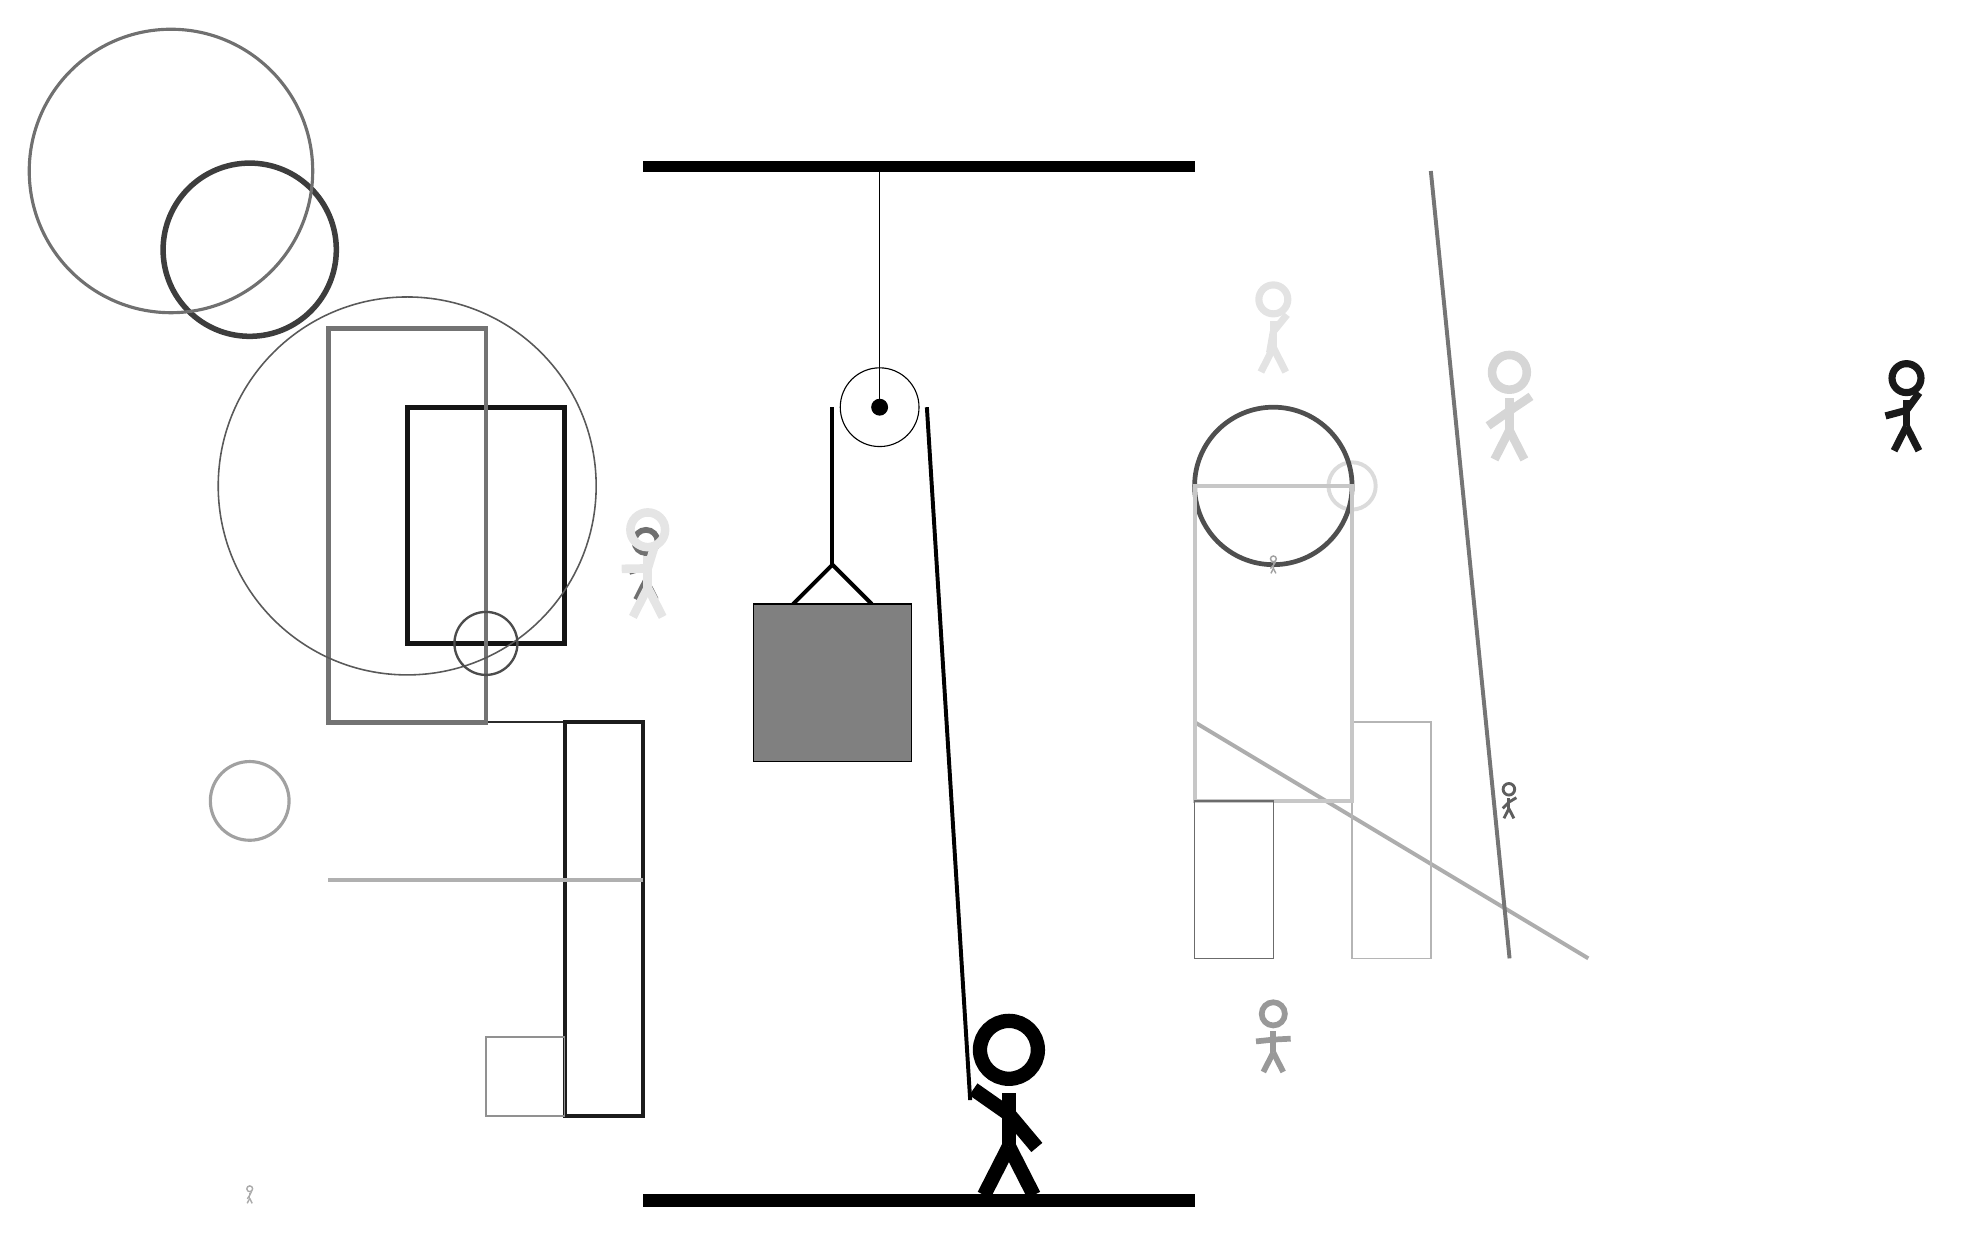
\begin{tikzpicture}
		%%%%% START %%%%%
		
		\draw[fill=black] (-2, 10) rectangle (5, 10.125);
		
		\draw (1, 7) circle (0.5);
		\draw[fill=black] (1, 7) circle (0.1);
		\draw (1, 10) -- (1, 7);
		
		\draw[line width=0.5mm] (-0.1, 4.5) -- (0.4, 5.0) -- (0.9, 4.5);
		\draw[fill=black!50] (-0.6, 4.5) rectangle (1.4, 2.5);
		
		\draw[line width=0.5mm] (0.4, 7) -- (0.4, 5.0);
		\centerarc[line width=0.5mm](1, 7)(0:180:0.6);
		\draw[line width=0.5mm](1.6, 7) -- (2.15, -1.8);
		
		\node at (2.6, -1.9) {\Strichmaxerl[10][-35][-50]};
		
		\draw[line width=0.2mm, color=black!83] (-2, 3) rectangle (-5, 3);
		
		\draw[line width=0.5mm, color=black!89] (-3, 3) rectangle (-2, -2);
		\node[line width=0.3mm, color=black!40] at (6, -1) {\Strichmaxerl[4][6][3]};
		\node[line width=0.4mm, color=black!90] at (14, 7) {\Strichmaxerl[5][15][54]};
		
		\draw[line width=0.5mm, color=black!51](7, 6) -- (7, 3);
		
		\draw[line width=0.5mm, color=black!80](5, 10) -- (5, 10);
		
		\draw [line width=0.5mm, color=black!14](7, 6) circle (0.3);
		\draw[line width=0.6mm, color=black!92] (-3, 4) rectangle (-5, 7);
		\node[line width=0.5mm, color=black!56] at (-2, 5) {\Strichmaxerl[4][16][87]};
		\draw[line width=0.5mm, color=black!32](10, 0) -- (5, 3);
		\node[line width=0.7mm, color=black!10] at (-2, 5) {\Strichmaxerl[6][1][73]};
		\draw [line width=0.7mm, color=black!76](-7, 9) circle (1.1);
		\draw[line width=0.2mm, color=black!43] (-3, -2) rectangle (-4, -1);
		
		\draw[line width=0.6mm, color=black!55] (-4, 8) rectangle (-6, 3);
		\draw [line width=0.6mm, color=black!69](6, 6) circle (1.0);
		\node[line width=0.6mm, color=black!11] at (6, 8) {\Strichmaxerl[5][80][51]};
		
		\draw[line width=0.2mm, color=black!29] (7, 0) rectangle (8, 3);
		\node[line width=0.6mm, color=black!37] at (6, 5) {\Strichmaxerl[1][46][58]};
		\node[line width=0.3mm, color=black!16] at (9, 7) {\Strichmaxerl[6][35][34]};
		\draw[line width=0.5mm, color=black!22] (5, 6) rectangle (7, 2);
		\node[line width=0.2mm, color=black!63] at (9, 2) {\Strichmaxerl[2][45][31]};
		
		\draw [line width=0.2mm, color=black!65](-5, 6) circle (2.4);
		\draw [line width=0.4mm, color=black!56](-8, 10) circle (1.8);
		\draw[line width=0.5mm, color=black!31](-2, 1) -- (-6, 1);
		\draw [line width=0.3mm, color=black!70](-4, 4) circle (0.4);
		
		\draw[line width=0.5mm, color=black!54](9, 0) -- (8, 10);
		\draw [line width=0.4mm, color=black!37](-7, 2) circle (0.5);
		\node[line width=0.5mm, color=black!33] at (-7, -3) {\Strichmaxerl[1][57][64]};
		\draw[line width=0.2mm, color=black!58] (6, 2) rectangle (5, 0);
		
		\draw[fill=black] (-2, -3) rectangle (5, -3.15);
		
		%%%%% END %%%%%
	\end{tikzpicture}
\end{document}